% Options for packages loaded elsewhere
\PassOptionsToPackage{unicode}{hyperref}
\PassOptionsToPackage{hyphens}{url}
\documentclass[
]{article}
\usepackage{xcolor}
\usepackage{amsmath,amssymb}
\setcounter{secnumdepth}{5}
\usepackage{iftex}
\ifPDFTeX
  \usepackage[T1]{fontenc}
  \usepackage[utf8]{inputenc}
  \usepackage{textcomp} % provide euro and other symbols
\else % if luatex or xetex
  \usepackage{unicode-math} % this also loads fontspec
  \defaultfontfeatures{Scale=MatchLowercase}
  \defaultfontfeatures[\rmfamily]{Ligatures=TeX,Scale=1}
\fi
\usepackage{lmodern}
\ifPDFTeX\else
  % xetex/luatex font selection
\fi
% Use upquote if available, for straight quotes in verbatim environments
\IfFileExists{upquote.sty}{\usepackage{upquote}}{}
\IfFileExists{microtype.sty}{% use microtype if available
  \usepackage[]{microtype}
  \UseMicrotypeSet[protrusion]{basicmath} % disable protrusion for tt fonts
}{}
\makeatletter
\@ifundefined{KOMAClassName}{% if non-KOMA class
  \IfFileExists{parskip.sty}{%
    \usepackage{parskip}
  }{% else
    \setlength{\parindent}{0pt}
    \setlength{\parskip}{6pt plus 2pt minus 1pt}}
}{% if KOMA class
  \KOMAoptions{parskip=half}}
\makeatother
\usepackage{color}
\usepackage{fancyvrb}
\newcommand{\VerbBar}{|}
\newcommand{\VERB}{\Verb[commandchars=\\\{\}]}
\DefineVerbatimEnvironment{Highlighting}{Verbatim}{commandchars=\\\{\}}
% Add ',fontsize=\small' for more characters per line
\newenvironment{Shaded}{}{}
\newcommand{\AlertTok}[1]{\textcolor[rgb]{1.00,0.00,0.00}{\textbf{#1}}}
\newcommand{\AnnotationTok}[1]{\textcolor[rgb]{0.38,0.63,0.69}{\textbf{\textit{#1}}}}
\newcommand{\AttributeTok}[1]{\textcolor[rgb]{0.49,0.56,0.16}{#1}}
\newcommand{\BaseNTok}[1]{\textcolor[rgb]{0.25,0.63,0.44}{#1}}
\newcommand{\BuiltInTok}[1]{\textcolor[rgb]{0.00,0.50,0.00}{#1}}
\newcommand{\CharTok}[1]{\textcolor[rgb]{0.25,0.44,0.63}{#1}}
\newcommand{\CommentTok}[1]{\textcolor[rgb]{0.38,0.63,0.69}{\textit{#1}}}
\newcommand{\CommentVarTok}[1]{\textcolor[rgb]{0.38,0.63,0.69}{\textbf{\textit{#1}}}}
\newcommand{\ConstantTok}[1]{\textcolor[rgb]{0.53,0.00,0.00}{#1}}
\newcommand{\ControlFlowTok}[1]{\textcolor[rgb]{0.00,0.44,0.13}{\textbf{#1}}}
\newcommand{\DataTypeTok}[1]{\textcolor[rgb]{0.56,0.13,0.00}{#1}}
\newcommand{\DecValTok}[1]{\textcolor[rgb]{0.25,0.63,0.44}{#1}}
\newcommand{\DocumentationTok}[1]{\textcolor[rgb]{0.73,0.13,0.13}{\textit{#1}}}
\newcommand{\ErrorTok}[1]{\textcolor[rgb]{1.00,0.00,0.00}{\textbf{#1}}}
\newcommand{\ExtensionTok}[1]{#1}
\newcommand{\FloatTok}[1]{\textcolor[rgb]{0.25,0.63,0.44}{#1}}
\newcommand{\FunctionTok}[1]{\textcolor[rgb]{0.02,0.16,0.49}{#1}}
\newcommand{\ImportTok}[1]{\textcolor[rgb]{0.00,0.50,0.00}{\textbf{#1}}}
\newcommand{\InformationTok}[1]{\textcolor[rgb]{0.38,0.63,0.69}{\textbf{\textit{#1}}}}
\newcommand{\KeywordTok}[1]{\textcolor[rgb]{0.00,0.44,0.13}{\textbf{#1}}}
\newcommand{\NormalTok}[1]{#1}
\newcommand{\OperatorTok}[1]{\textcolor[rgb]{0.40,0.40,0.40}{#1}}
\newcommand{\OtherTok}[1]{\textcolor[rgb]{0.00,0.44,0.13}{#1}}
\newcommand{\PreprocessorTok}[1]{\textcolor[rgb]{0.74,0.48,0.00}{#1}}
\newcommand{\RegionMarkerTok}[1]{#1}
\newcommand{\SpecialCharTok}[1]{\textcolor[rgb]{0.25,0.44,0.63}{#1}}
\newcommand{\SpecialStringTok}[1]{\textcolor[rgb]{0.73,0.40,0.53}{#1}}
\newcommand{\StringTok}[1]{\textcolor[rgb]{0.25,0.44,0.63}{#1}}
\newcommand{\VariableTok}[1]{\textcolor[rgb]{0.10,0.09,0.49}{#1}}
\newcommand{\VerbatimStringTok}[1]{\textcolor[rgb]{0.25,0.44,0.63}{#1}}
\newcommand{\WarningTok}[1]{\textcolor[rgb]{0.38,0.63,0.69}{\textbf{\textit{#1}}}}
\usepackage{longtable,booktabs,array}
\usepackage{calc} % for calculating minipage widths
% Correct order of tables after \paragraph or \subparagraph
\usepackage{etoolbox}
\makeatletter
\patchcmd\longtable{\par}{\if@noskipsec\mbox{}\fi\par}{}{}
\makeatother
% Allow footnotes in longtable head/foot
\IfFileExists{footnotehyper.sty}{\usepackage{footnotehyper}}{\usepackage{footnote}}
\makesavenoteenv{longtable}
\usepackage{graphicx}
\makeatletter
\newsavebox\pandoc@box
\newcommand*\pandocbounded[1]{% scales image to fit in text height/width
  \sbox\pandoc@box{#1}%
  \Gscale@div\@tempa{\textheight}{\dimexpr\ht\pandoc@box+\dp\pandoc@box\relax}%
  \Gscale@div\@tempb{\linewidth}{\wd\pandoc@box}%
  \ifdim\@tempb\p@<\@tempa\p@\let\@tempa\@tempb\fi% select the smaller of both
  \ifdim\@tempa\p@<\p@\scalebox{\@tempa}{\usebox\pandoc@box}%
  \else\usebox{\pandoc@box}%
  \fi%
}
% Set default figure placement to htbp
\def\fps@figure{htbp}
\makeatother
\setlength{\emergencystretch}{3em} % prevent overfull lines
\providecommand{\tightlist}{%
  \setlength{\itemsep}{0pt}\setlength{\parskip}{0pt}}
\usepackage{bookmark}
\IfFileExists{xurl.sty}{\usepackage{xurl}}{} % add URL line breaks if available
\urlstyle{same}
\hypersetup{
  hidelinks,
  pdfcreator={LaTeX via pandoc}}

\author{}
\date{}

\begin{document}

\begin{titlepage}
\centering
\vspace*{2.5cm}

{\LARGE \textbf{Team 4}}\\[0.4cm]
{\Large Chrome Extension Threat \& Risk Analyzer (CETRA)}\\[1.2cm]

\rule{0.8\textwidth}{0.5pt}\\[0.8cm]

\textbf{Group Members}\\[0.4cm]

Kevin Deshayes — \texttt{kede23@student.bth.se}\\
Fajer Alhamwi — \texttt{faaa22@student.bth.se}\\
Majid Mohamed Hamid — \texttt{mamd15@student.bth.se}\\
Hugo Jonsson — \texttt{hujo23@student.bth.se}\\
Kasper Thunell — \texttt{katu22@student.bth.se}\\
Theo Svensson — \texttt{thsn23@student.bth.se}\\

\vfill
{\large DV1512}\\
{\large \today}

\end{titlepage}

\tableofcontents
\newpage

{
\setcounter{tocdepth}{3}
\tableofcontents
}
\section{CETRA Documentation}\label{cetra-documentation}

This folder contains the documentation required for the DV1512
submission.

\subsection{Contents}\label{contents}

\begin{itemize}
\tightlist
\item
  \href{architecture.md}{Architecture Description}
\item
  \href{api.md}{API Documentation}
\item
  \href{requirements.md}{Requirements and Scope}
\item
  \href{dependencies.md}{Dependencies}
\item
  \href{prerequisites.md}{Prerequisites}
\item
  \href{deployment.md}{Deployment Guide (Build \& Run)}
\item
  \href{user-guide.md}{User Guide}
\item
  \href{threat-modeling.md}{Threat Modeling}
\item
  \href{vulnerability-scanning.md}{Vulnerability Scanning}
\end{itemize}

\subsection{Diagrams and Models}\label{diagrams-and-models}

\begin{itemize}
\tightlist
\item
  Diagrams: \texttt{docs/diagrams/}
\item
  UML/PlantUML: \texttt{docs/uml/}
\end{itemize}

\subsection{Architecture Diagram}\label{architecture-diagram}

The following diagram shows the high-level component architecture of
CETRA, including the frontend container, backend services, database, and
external analysis systems.

\begin{figure}
\centering
\pandocbounded{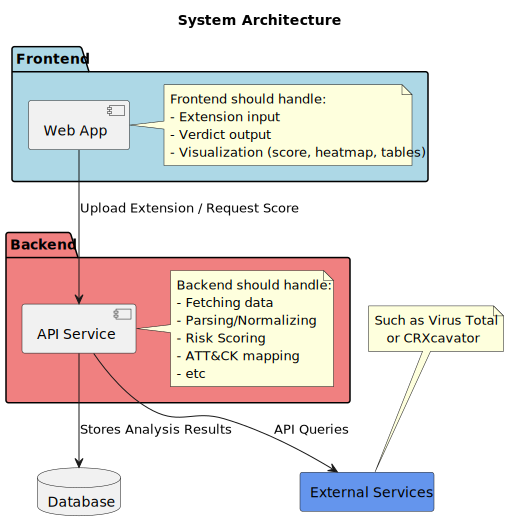
\includegraphics[keepaspectratio]{diagrams/architecture.png}}
\caption{CETRA Component Architecture}
\end{figure}

The architecture diagram was created using PlantUML and follows a
C4-style component diagram approach.

\section{API Documentation}\label{api-documentation}

\subsection{Overview}\label{overview}

CETRA does not expose a public API. All application functionality is
accessed through a Django-based Web UI. Internal endpoints coordinate
extension analysis, report generation, and data retrieval.

\begin{center}\rule{0.5\linewidth}{0.5pt}\end{center}

\subsection{Authentication}\label{authentication}

Authentication is handled using Django's built-in authentication
mechanism. Access to analysis functionality and stored reports is
restricted to authenticated users.

\begin{center}\rule{0.5\linewidth}{0.5pt}\end{center}

\subsection{Internal Application Endpoints
(High-Level)}\label{internal-application-endpoints-high-level}

\begin{itemize}
\tightlist
\item
  \textbf{Extension Submission}

  \begin{itemize}
  \tightlist
  \item
    Accepts Chrome Web Store IDs, ZIP files, or CRX files
  \item
    Initiates the analysis workflow through the backend API router
  \end{itemize}
\item
  \textbf{Report Retrieval}

  \begin{itemize}
  \tightlist
  \item
    Displays stored analysis results in the Web UI
  \item
    Supports exporting reports in JSON format
  \end{itemize}
\item
  \textbf{MITRE ATT\&CK Analysis}

  \begin{itemize}
  \tightlist
  \item
    Initiates behavior mapping based on sandbox analysis results
  \item
    Displays tactics and techniques through the Web UI
  \end{itemize}
\end{itemize}

\begin{center}\rule{0.5\linewidth}{0.5pt}\end{center}

\subsection{External APIs}\label{external-apis}

The system integrates with the following external services:

\begin{itemize}
\tightlist
\item
  \textbf{VirusTotal API} -- malware detection and reputation analysis
\item
  \textbf{OPSWAT MetaDefender API} -- multi-engine malware scanning
\item
  \textbf{SecureAnnex API} -- sandbox-based behavioral analysis
\item
  \textbf{Google Gemini API} -- AI-assisted interpretation of findings
\end{itemize}

API credentials are provided via environment variables.

\section{Requirements and Scope}\label{requirements-and-scope}

\subsection{Functional Requirements}\label{functional-requirements}

The CETRA system fulfills the following functional requirements:

\begin{itemize}
\tightlist
\item
  The system accepts uploaded Chrome extensions for analysis.
\item
  The system extracts an extension ID from uploaded data.
\item
  The system submits scan requests to multiple external analysis
  services.
\item
  The system aggregates results from multiple scanners.
\item
  The system generates an analysis report.
\item
  The system retrieves stored reports for later viewing.
\item
  The system persists analysis results in a database.
\item
  The system requires authentication to access the application,
  including generating and viewing analysis reports.
\end{itemize}

\begin{center}\rule{0.5\linewidth}{0.5pt}\end{center}

\subsection{Non-Functional
Requirements}\label{non-functional-requirements}

The system is designed to satisfy the following non-functional
requirements:

\begin{itemize}
\tightlist
\item
  The system uses a modular, component-based architecture.
\item
  The system supports integration with multiple external APIs.
\item
  The system isolates untrusted file analysis from the core system.
\item
  The system enforces authorization at the application level so that
  only authenticated users can access stored analysis reports.
\item
  The system remains usable while long-running analyses are performed.
\item
  The system validates uploaded files as Chrome extensions (e.g.,
  presence and structure of \texttt{manifest.json}) and rejects invalid
  uploads.
\item
  The system reduces supply-chain risk by restricting analysis inputs to
  Chrome Web Store extensions only.
\end{itemize}

\begin{center}\rule{0.5\linewidth}{0.5pt}\end{center}

\subsection{Security Scope and
Limitations}\label{security-scope-and-limitations}

The system enforces authentication and authorization at the application
level. Analysis results are stored in a local SQLite database, which is
not encrypted at rest.

As a result, users with direct operating system access to the host
machine may read database contents outside of the application. Passwords
are stored using secure cryptographic hashing.

Protecting data at rest (e.g., database encryption and OS-level access
control) is considered out of scope for the current prototype and would
be required for a production deployment.

\section{Dependencies}\label{dependencies}

\begin{itemize}
\tightlist
\item
  Linux OS (native, WSL, or virtual machine)
\item
  Python 3.x
\item
  pip
\item
  Python packages listed in \texttt{requirements.txt}
\item
  External tools used during analysis:

  \begin{itemize}
  \tightlist
  \item
    OWASP ZAP
  \item
    OWASP Threat Dragon
  \end{itemize}
\end{itemize}

\section{Prerequisites}\label{prerequisites}

The application relies on external malware analysis APIs and an AI
module. To enable these integrations, create a \texttt{.env} file (based
on \texttt{.env.example}) and provide valid API keys:

\begin{itemize}
\tightlist
\item
  VirusTotal API key: https://www.virustotal.com
\item
  OPSWAT MetaDefender API key: https://id.opswat.com/login
\item
  SecureAnnex API key: https://app.secureannex.com/login
\item
  Google Gemini API key (AI module):
  https://aistudio.google.com/app/api-keys
\end{itemize}

Make sure all required API keys are inserted before running the system,
as several components depend on them.

\section{Deployment Guide (Build \&
Run)}\label{deployment-guide-build-run}

This document describes how to deploy and run the CETRA application from
source in a development environment.

The instructions assume a Linux-based system (native Linux, WSL, or
virtual machine).

\begin{center}\rule{0.5\linewidth}{0.5pt}\end{center}

\subsection{1. Dependencies}\label{dependencies-1}

See \texttt{docs/dependencies.md}.

\subsection{2. Prerequisites (.env)}\label{prerequisites-.env}

See \texttt{docs/prerequisites.md}.

\subsection{3. Install Dependencies}\label{install-dependencies}

Install the required Python packages using pip:

\begin{Shaded}
\begin{Highlighting}[]
\ExtensionTok{pip}\NormalTok{ install }\AttributeTok{{-}r}\NormalTok{ requirements.txt}
\end{Highlighting}
\end{Shaded}

\subsection{4. Setup \& Run}\label{setup-run}

\begin{enumerate}
\def\labelenumi{\arabic{enumi}.}
\tightlist
\item
  \textbf{Migrate Database}: Run \texttt{python\ manage.py\ migrate} to
  apply changes to the database.
\item
  \textbf{Run Tests (Optional)}: Run \texttt{python\ manage.py\ test} to
  ensure the system is stable.
\item
  \textbf{Create User}: Execute
  \texttt{python\ manage.py\ createsuperuser\ -\/-username=joe\ -\/-email=joe@example.com}
  to create a user in the Django database.

  \begin{itemize}
  \tightlist
  \item
    Follow the terminal instructions.
  \item
    Bypass password strength validation when prompted.
  \end{itemize}
\item
  \textbf{Start Server}: Run \texttt{python\ manage.py\ runserver} to
  launch the program.

  \begin{itemize}
  \tightlist
  \item
    Open your browser to the localhost address (usually
    http://127.0.0.1:8000).
  \item
    Log in with the credentials you entered during the
    \texttt{createsuperuser} step.
  \end{itemize}
\item
  \textbf{Security Note}: For security, too many incorrect login
  attempts will trigger a temporary lockout with a 60-second countdown
  before you can try again.
\end{enumerate}

\section{User Guide}\label{user-guide}

This document describes how to use CETRA (Chrome Extension Threat \&
Risk Analyzer) from an end-user perspective.

\begin{center}\rule{0.5\linewidth}{0.5pt}\end{center}

\subsection{Intended Users and Use
Cases}\label{intended-users-and-use-cases}

CETRA is designed for anyone who wants to assess the security and
trustworthiness of Chrome extensions.

Typical users include:

\begin{itemize}
\tightlist
\item
  \textbf{End users} who want to verify whether a Chrome extension is
  safe to install.
\item
  \textbf{Students} learning about software security and malware
  analysis.
\item
  \textbf{Security analysts} investigating extension permissions, risks,
  and behavior.
\item
  \textbf{Developers} who want to inspect what their own extensions
  expose.
\end{itemize}

\begin{center}\rule{0.5\linewidth}{0.5pt}\end{center}

\subsection{Getting Started}\label{getting-started}

To use CETRA, the application must be running and the user must be
authenticated. Refer to the Deployment Guide for setup instructions.

Once logged in, the user is presented with the main navigation
interface.

\begin{center}\rule{0.5\linewidth}{0.5pt}\end{center}

\subsection{Submitting an Extension for
Analysis}\label{submitting-an-extension-for-analysis}

The \textbf{Home} page serves as the primary analysis interface.

Users can submit a Chrome extension using one of the following methods:

\begin{itemize}
\tightlist
\item
  \textbf{Chrome Web Store ID}
\item
  \textbf{ZIP file}
\item
  \textbf{CRX file}
\end{itemize}

After submission, the system validates the input and initiates the
analysis workflow.

If a report for the same extension exists from the last 30 days, the
user may choose to either: - Open the existing report, or - Run a new
analysis

Analysis typically takes a few minutes to complete.

\begin{center}\rule{0.5\linewidth}{0.5pt}\end{center}

\subsection{Viewing Analysis Results}\label{viewing-analysis-results}

Once the analysis is complete, CETRA presents a detailed result view
including:

\begin{itemize}
\tightlist
\item
  Overall verdict and threat score
\item
  Requested permissions
\item
  Findings from external analysis services
\item
  Malware family and category information
\end{itemize}

The system aggregates results from multiple sources to provide a unified
view.

\begin{center}\rule{0.5\linewidth}{0.5pt}\end{center}

\subsection{History and Report
Management}\label{history-and-report-management}

The \textbf{History} tab allows users to:

\begin{itemize}
\tightlist
\item
  View previously analyzed extensions
\item
  Browse results using pagination
\item
  Download analysis reports in JSON format
\end{itemize}

This enables users to retain and reuse analysis results for later
review.

\begin{center}\rule{0.5\linewidth}{0.5pt}\end{center}

\subsection{MITRE ATT\&CK Analysis}\label{mitre-attck-analysis}

The \textbf{MITRE ATT\&CK} tab provides deeper behavioral analysis.

For supported reports, users can: - Initiate MITRE ATT\&CK mapping -
View detected tactics and techniques - Track analysis status (Not
Started, Completed, Not Available)

MITRE analysis is based on sandbox and behavioral data from external
services.

\begin{center}\rule{0.5\linewidth}{0.5pt}\end{center}

\subsection{Settings and Interface
Features}\label{settings-and-interface-features}

The \textbf{Settings} page allows users to:

\begin{itemize}
\tightlist
\item
  Toggle between light and dark mode themes
\item
  Adjust basic user interface preferences
\end{itemize}

Users can log out securely at any time using the logout option in the
navigation bar.

\begin{center}\rule{0.5\linewidth}{0.5pt}\end{center}

\subsection{Security Notes}\label{security-notes}

\begin{itemize}
\tightlist
\item
  Authentication is required to access all analysis and reporting
  functionality.
\item
  Multiple failed login attempts will trigger a temporary lockout with a
  cooldown period to reduce brute-force attempts.
\end{itemize}

\begin{center}\rule{0.5\linewidth}{0.5pt}\end{center}

\subsection{Summary}\label{summary}

Using CETRA consists of submitting a Chrome extension, waiting for the
analysis to complete, and reviewing the aggregated results. The system
is designed to be simple to use while providing meaningful security
insights into Chrome extensions.

\section{Threat Modeling}\label{threat-modeling}

\subsection{Overview}\label{overview-1}

Threat modeling was performed to identify and assess potential security
threats to the CETRA system. The analysis focused on user input, the Web
UI, backend API routing, and external API integrations.

The threat modeling process was conducted using OWASP Threat Dragon and
follows a STRIDE-based approach.

\begin{center}\rule{0.5\linewidth}{0.5pt}\end{center}

\subsection{Identified Threats and
Mitigations}\label{identified-threats-and-mitigations}

\subsubsection{User Input}\label{user-input}

\paragraph{Denial of Service (DDoS)}\label{denial-of-service-ddos}

\begin{itemize}
\tightlist
\item
  \textbf{Threat Type:} Denial of Service
\item
  \textbf{Description:} An attacker may attempt to overwhelm the system
  by submitting excessive files or requests.
\item
  \textbf{Mitigation:} The system restricts users to submitting only one
  file at a time.
\item
  \textbf{Risk Score:} 59 (Medium)
\end{itemize}

\paragraph{SQL Injection}\label{sql-injection}

\begin{itemize}
\tightlist
\item
  \textbf{Threat Type:} Tampering
\item
  \textbf{Description:} Malicious input could be used to manipulate SQL
  queries.
\item
  \textbf{Mitigation:} Input validation is enforced.
\item
  \textbf{Risk Score:} 80 (High)
\end{itemize}

\paragraph{SQL Injection --
Authentication}\label{sql-injection-authentication}

\begin{itemize}
\tightlist
\item
  \textbf{Threat Type:} Tampering / Authentication Bypass
\item
  \textbf{Description:} Improper input handling may allow bypassing
  authentication.
\item
  \textbf{Mitigation:} Input validation is enforced.
\item
  \textbf{Risk Score:} 80 (High)
\end{itemize}

\begin{center}\rule{0.5\linewidth}{0.5pt}\end{center}

\subsubsection{Web UI Frontend}\label{web-ui-frontend}

\paragraph{Spoofing}\label{spoofing}

\begin{itemize}
\tightlist
\item
  \textbf{Threat Type:} Spoofing
\item
  \textbf{Description:} Potential spoofing attempts against the
  frontend.
\item
  \textbf{Mitigation:} Considered non-threatening as the software is not
  publicly deployed.
\item
  \textbf{Risk Score:} 10 (Low)
\end{itemize}

\paragraph{Server Information
Disclosure}\label{server-information-disclosure}

\begin{itemize}
\tightlist
\item
  \textbf{Threat Type:} Information Disclosure
\item
  \textbf{Description:} Server version information may be leaked via
  HTTP headers.
\item
  \textbf{Mitigation:} Server configuration can be modified to remove or
  obfuscate identifying headers.
\item
  \textbf{Risk Score:} 10 (Low)
\end{itemize}

\begin{center}\rule{0.5\linewidth}{0.5pt}\end{center}

\subsubsection{API Router}\label{api-router}

\paragraph{File Download Information
Disclosure}\label{file-download-information-disclosure}

\begin{itemize}
\tightlist
\item
  \textbf{Threat Type:} Information Disclosure
\item
  \textbf{Description:} Improper file handling may expose sensitive
  files.
\item
  \textbf{Mitigation:} Files should be validated before being
  downloaded.
\item
  \textbf{Risk Score:} 20 (Low)
\end{itemize}

\begin{center}\rule{0.5\linewidth}{0.5pt}\end{center}

\subsubsection{API Interfaces}\label{api-interfaces}

\paragraph{Man-in-the-Middle (MITM)}\label{man-in-the-middle-mitm}

\begin{itemize}
\tightlist
\item
  \textbf{Threat Type:} Tampering
\item
  \textbf{Description:} External API responses may be altered during
  transmission.
\item
  \textbf{Mitigation:} API results should be validated before use.
\item
  \textbf{Risk Score:} 40 (Low)
\end{itemize}

\begin{center}\rule{0.5\linewidth}{0.5pt}\end{center}

\subsection{Risk Assessment}\label{risk-assessment}

Risk levels were assessed using CVSS v4.0 scoring where applicable.
High-risk threats were identified pr

\section{Vulnerability Scanning}\label{vulnerability-scanning}

\subsection{Overview}\label{overview-2}

Security testing was performed to identify vulnerabilities in the CETRA
Web UI. The testing focused on detecting common web application
vulnerabilities and misconfigurations.

\begin{center}\rule{0.5\linewidth}{0.5pt}\end{center}

\subsection{Tooling}\label{tooling}

\begin{itemize}
\tightlist
\item
  \textbf{Tool:} OWASP ZAP
\item
  \textbf{Target:} CETRA Web UI (local development instance)
\end{itemize}

\begin{center}\rule{0.5\linewidth}{0.5pt}\end{center}

\subsection{Scan Context and Authentication
Scope}\label{scan-context-and-authentication-scope}

OWASP ZAP scanning was performed against an authenticated session of the
CETRA Web UI. Authentication was required in order to access protected
functionality, such as submitting extensions for analysis and viewing
stored reports.

Unauthenticated scanning was not sufficient to exercise the full attack
surface, as the application enforces access control on core
functionality.

As a result, all identified SQL injection findings were discovered in an
authenticated context. The authentication mechanism therefore mitigates
the risk of unauthenticated exploitation. However, these findings remain
valid, as SQL injection vulnerabilities can still be exploited by an
authenticated attacker if proper query handling and input validation are
not enforced.

\subsection{Identified
Vulnerabilities}\label{identified-vulnerabilities}

\subsubsection{High Severity}\label{high-severity}

\begin{longtable}[]{@{}lll@{}}
\toprule\noalign{}
Vulnerability & Severity & Count \\
\midrule\noalign{}
\endhead
\bottomrule\noalign{}
\endlastfoot
SQL Injection & High & 4 \\
SQL Injection -- Authentication Bypass & High & 4 \\
\end{longtable}

\subsubsection{Medium Severity}\label{medium-severity}

\begin{longtable}[]{@{}lll@{}}
\toprule\noalign{}
Vulnerability & Severity & Count \\
\midrule\noalign{}
\endhead
\bottomrule\noalign{}
\endlastfoot
Content Security Policy (CSP) Header Not Set & Medium & 14 \\
\end{longtable}

\subsubsection{Low Severity}\label{low-severity}

\begin{longtable}[]{@{}
  >{\raggedright\arraybackslash}p{(\linewidth - 4\tabcolsep) * \real{0.8000}}
  >{\raggedright\arraybackslash}p{(\linewidth - 4\tabcolsep) * \real{0.1231}}
  >{\raggedright\arraybackslash}p{(\linewidth - 4\tabcolsep) * \real{0.0769}}@{}}
\toprule\noalign{}
\begin{minipage}[b]{\linewidth}\raggedright
Vulnerability
\end{minipage} & \begin{minipage}[b]{\linewidth}\raggedright
Severity
\end{minipage} & \begin{minipage}[b]{\linewidth}\raggedright
Count
\end{minipage} \\
\midrule\noalign{}
\endhead
\bottomrule\noalign{}
\endlastfoot
Cookie No HttpOnly Flag & Low & 10 \\
Server Leaks Version Information via ``Server'' Header & Low & 17 \\
X-Content-Type-Options Header Missing & Low & 1 \\
\end{longtable}

\subsubsection{Informational}\label{informational}

\begin{longtable}[]{@{}ll@{}}
\toprule\noalign{}
Finding & Count \\
\midrule\noalign{}
\endhead
\bottomrule\noalign{}
\endlastfoot
Authentication Request Identified & 4 \\
Session Management Response Identified & 12 \\
User Agent Fuzzer & 153 \\
\end{longtable}

\begin{center}\rule{0.5\linewidth}{0.5pt}\end{center}

\subsection{High-Severity Vulnerabilities: Mitigation and
Justification}\label{high-severity-vulnerabilities-mitigation-and-justification}

\subsubsection{SQL Injection}\label{sql-injection-1}

\begin{itemize}
\tightlist
\item
  \textbf{Description:} User-controlled input may be used to inject
  malicious SQL queries.
\item
  \textbf{Impact:} Unauthorized access to or manipulation of stored
  data.
\item
  \textbf{Mitigation:}

  \begin{itemize}
  \tightlist
  \item
    Enforce strict server-side input validation.
  \item
    Use parameterized queries for all database operations.
  \item
    Restrict access to vulnerable endpoints through authentication and
    authorization mechanisms.
  \end{itemize}
\item
  \textbf{Status:} Identified in an authenticated scan context;
  mitigation is required before production deployment.
\end{itemize}

\begin{center}\rule{0.5\linewidth}{0.5pt}\end{center}

\subsubsection{SQL Injection -- Authentication
Bypass}\label{sql-injection-authentication-bypass}

\begin{itemize}
\tightlist
\item
  \textbf{Description:} Improper query handling may allow attackers to
  bypass authentication mechanisms.
\item
  \textbf{Impact:} Unauthorized access to protected functionality and
  stored reports.
\item
  \textbf{Mitigation:}

  \begin{itemize}
  \tightlist
  \item
    Enforce strict server-side input validation.
  \item
    Ensure authentication and authorization checks occur before database
    queries on protected routes.
  \item
    Use parameterized queries to prevent query manipulation.
  \end{itemize}
\item
  \textbf{Status:} Identified in an authenticated scan context; the
  authentication mechanism mitigates unauthenticated exploitation, but
  mitigation is required before production deployment.
\end{itemize}

\begin{center}\rule{0.5\linewidth}{0.5pt}\end{center}

\subsection{Summary}\label{summary-1}

\begin{itemize}
\tightlist
\item
  \textbf{Total identified vulnerabilities and threats:} 13
\item
  \textbf{Mitigated vulnerabilities and threats:} 7
\item
  \textbf{Residual vulnerabilities and threats:} 6
\end{itemize}

The remaining residual vulnerabilities are considered acceptable within
the scope of the prototype and do not pose a critical risk in a
controlled development environment.

\begin{center}\rule{0.5\linewidth}{0.5pt}\end{center}

\subsection{Known Limitations and Future
Work}\label{known-limitations-and-future-work}

\begin{itemize}
\tightlist
\item
  Lack of in-house malware analysis and verdict generation.
\item
  Heavy reliance on external services such as VirusTotal.
\item
  Future improvements include containerization and implementing
  structured return values to enable pipeline-based execution.
\end{itemize}

\begin{center}\rule{0.5\linewidth}{0.5pt}\end{center}

\subsection{Conclusion}\label{conclusion}

CETRA provides a valid foundational prototype for further development.
The security analysis highlights areas requiring hardening before
production deployment, while demonstrating a solid understanding of
threat modeling and vulnerability management principles.

\end{document}
